\section{Implementation}
\label{sec:impl}

We implemented an iterative version of Algorithm~\ref{alg:search} with
stratified search using Python. The system diagram is shown in
Figure~\ref{fig:system}. The core of the system implements the state machine
abstractions and common searching functionality. The implementation is in a
modular manner such that the heuristic constraints and state machine
specifications can be easily added without modifying the core logic.



Next, we briefly describe the key components and major implementation decisions.

\subsection{State Machine}

The state transition diagram is represented using adjacent list of
\texttt{Transition} objects. Each \texttt{Transition} object represents an edge
in the transition graph, and consists of: (1) source and destination state, (2)
a \texttt{pkt\_spec} function, (3) clock guard and (4) the set of clock
variables to be reset along with this transition, in which (3) and (4) are
optional.

The \texttt{pkt\_spec} function takes the current state and  a packet as input,
and returns \texttt{true} if the packet should trigger the corresponding
transition. As mentioned in Section~\ref{subsec:basic}, the packet payload is
of no interest, thus the \texttt{pkt\_spec} function typically just 
checks certain fields of the packet header, such as \texttt{type},
\texttt{subtype}, \texttt{is\_retry}, \texttt{seq\_num}, etc.  Additionally,
this function is also responsible to \textit{fabricate} a packet with the
desired header fields that are expected by the transition. This is to
facilitate the Type-1 transitions where we need to guess the missing packets.

The clock variable abstraction provides two interfaces: \texttt{reset()} and
\texttt{read()}. Note that the concept of time in the verification context is
with respect to the packet trace, not the wall time of the verification system.
Therefore, both the \texttt{reset()} and \texttt{read()} function takes a packet in
the trace as argument. When reset by a packet, the clock variable remembers the
timestamp of the last bit of the packet. When read with a packet, the variable
returns the elapsed time between its last reset timestamp and the first bit of
the packet. Finally, the clock guards are simply a boolean expression consisting
of the value read from clock variables and certain constants.

\begin{figure}[t!]
  \centering
  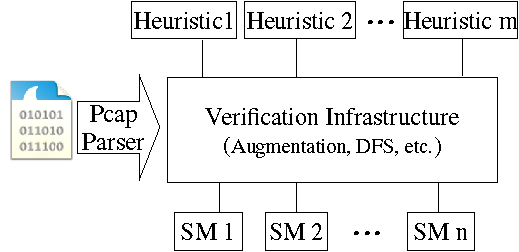
\includegraphics[width=0.4\textwidth]{./figures/system.pdf}
  \caption{\textbf{System Diagram.} The core verification logic is shared among all state
  machine instances.}
  \label{fig:system}
\end{figure}


A challenge arises about how to reset clock variables or check clock guards
with \textit{fabricated} packets, since their timestamps were not observed in
the trace but were synthesized. Given the discrete timestamp assumption, a straw
man approach may be to enumerate all possible timestamps for the
first and last bit of the fabricated packets. However, we note that it does not
make sense to synthesize timestamps which violates the clock guards, since the
packet is fabricated in the first place. In other words, we are only interested
in the type of packets missed, not their timestamps. Therefore, clock guards are
only checked between adjacent real packets, and clock variables are only reset
or read with real packets in the sniffer trace.


\subsection{Stratified Depth First Search}

We use the \texttt{TransitionTreeNode} object to track one step of the search
process.
%
Note that even the complete transition graph is a tree, only one \texttt{child}
pointer need to be stored, since at any instant only one branches of the tree is
explored due the iterative implementation.
%
The node maintains \texttt{visited}
flags of whether
each type of transition has been attempted to facilities the iterative DFS
process.
%
The node's timestamp is set to be the last bit of the packet that
triggers this transition.
%
This timestamp is used to calculate the available time should Type-1 transitions
be needed.

An interesting implementation decision is how to estimate the minimal duration
of each transition, which is used together with the available time before next
packet to limited the depth of Type-1 transitions. The duration should be the
maximum of two values: minimal elapsed time that meets the clock guard and
minimal duration of the packet that can trigger the transition. The former can
be easily obtained from the clock guards. Theoretically, the minimal packet
duration should be calculated assuming the shorted packet sent in the highest
bit rate. However, we found this assumption is often too conservative in
practice and causes many unnecessary Type-1 transitions. Therefore, we use an
Exponential Weighted Moving Average (EWMA) of the durations of previous packets
of the same type to estimate the duration of missing packets. To
accommodate sudden packet length or bit rate changes, we set the packet
duration to be EWMA divided a constant factor (4 in our implementation).

We implemented the stratified searching in a per packet manner. More
specifically, we try to consume each packet in stratified manner with threshold
$\{k_0, k_1,\ldots k_n\}$, $k_i < k_{i+1}$. When searching with threshold $k_i$
fails, we clear all previous nodes' \texttt{visited} flags and repeat the
searching with threshold $k_{i+1}$. If the search for the previous packet
succeed with threshold $k_i$, we start the next packet's search with $k_i$,
skipping the bootstrapping process. 
